\documentclass{llncs}
\usepackage{makeidx}
\setcounter{tocdepth}{2}
\title{Symbolic Music Similarity}
\author{Ali Bektas \and Paul Kröger}
\date{April 2020}


\usepackage{graphicx}
\graphicspath{{./img/}}

\usepackage{verbatim}
\usepackage{mathtools}

\setcounter{tocdepth}{2}
\pagestyle{plain}



\begin{document}

	
	\thispagestyle{empty}
   	\begin{center}	
		\vspace{100pt}
		\Huge Symbolic Melodic Music Similarity\\
		\vspace{5pt}
		\Large Similarity Search 2019-20\\
		\vspace{20pt}
		Ali Bektas\\
		Paul Kröger \\
		\vspace{150pt}
		\begin{figure}[h!]
			\centering
	        
\includegraphics[width=200px,height=100px,keepaspectratio]{hu-berlin-logo}
        \end{figure}
		\vspace{5pt}
		\Large{\today}
	\end{center}
	
	\newpage
	\tableofcontents
	

	\newpage
	\pagestyle{plain}
	\setcounter{page}{1}
	\begin{center}	

		\large{\textbf{Symbolic Melodic Music Similarity}}\\
		\vspace{5pt} 
		
		\small{Ali Bektas}\\
		\vspace{5pt}

		\small{Paul Kröger}\\
		\vspace{5pt}

		\small{\textbf{Advisor} : Prof. Dr. Ulf Leser}\\
		\vspace{5pt}

		\small{\today}
	\end{center}


	\tableofcontents
	
	\begin{abstract}
	In today's digitalized music industry the need to compare musical data in terms of their content the question of similarity between musical objects becomes a challenge. Because there 
	is not a single method to satisfy all needs, various approaches have been introduced to the field in recent decades. We introduce approaches which focus on symbolic melodic data, that is, a representation of the melody of a piece based on an alphabet of symbols. As the leading algorithms in this field, we examine J.Urbano's et al. algorithm which compares the shape of melodies and an algorithm by N.Orio et al. which constructs a tree out of melodies and uses the shortest path between them to determine similarity. Furthermore we will show how the MIREX competition handled the lack of an existing definition for similarity between pieces of music.
	\end{abstract}

	\section{Introduction}
		Similarity measures lie at the heart of Information Retrieval. This is also the case for music similarity. For a subscriber of a music streaming application like Spotify, Last.fm etc. to be recommended latest albums or for a researcher to find related pieces in a database, determining similarity between pieces of music is crucial. Symbolic Music Similarity algorithms are based on symbols that represent the data as input. Within Symbolic Music Similarity there are algorithms that deal with polyphonic data and others that deal with monophonic data. In this paper we will look at the field of Symbolic Melodic Music Similarity, that is , the algorithms which only focuses on monophonic data. 

        Since we are mainly concerned with Western music, we can restrict ourselves to 12 tones in an octave, other cultures however may use more or less notes. In Middle Eastern countries,for instance,there are 9 tones between two notes of a whole tone interval \cite{six}.

		In our paper we will follow the classification used by Velardo et al. \cite{two}. According to Velardo et al. a symbolic music similarity algorithm belongs to either of the four classes (1) Music Theory, (2) Cognition, (3) Mathematics or (4) Hybrid. Hybrid algorithms are usually formed by taking a linear combination of different similarity measures.
		
		We will introduce two algorithms to showcase how symbolic melodic data can be represented and compared :
		\begin{itemize}
		\item The system proposed by J. Urbano et al. \cite{five_point_five} forms spline-sequence for a query melody and compares it with other spline-sequences using a sequence alignment method to determine similarity between pieces. 
		\item In contrast, the approach by N.Orio et al. \cite{two_point_four} incorporates routines , that heavily depend on Music Theory, to generalize the melody, into simpler melodies while forming a tree structure. Within this tree the shortest path between given melodies is then found.

        After this we will introduce MIREX, the Music Information Retrieval Evaluation eXchange, that organizes annual competitions for researchers to test their algorithms against one another. We will explain how the subjectivity of music similarity in these competitions is reduced to a minimum by having experts establishing a Ground Truth. We will explain how this process takes place based on the example of the 2005 competition. The resulting data, against which the result of an algorithms is to be compared, manifest an (non-total) order which makes it more difficult for precision and recall measures to come to a meaningful result. We will explain how this problem is solved with a novel measure called Average Dynamic Recall.

        In Chapter 4 we will show how these algorithms perform with the Ground Truths from MIREX competitions.

        Finally, we will mention the strengths and weaknesses of each algorithm and how subjectivity of similarity prevents the field from establishing a unified algorithm , that satisfy     
	

		 
		
	\section{Algorithms}

		\subsection{A Graph Based Approach}

		Orio et al. \cite{two_point_four} introduce  a series of operations to transform a collection of music pieces into a single large tree. Pieces are first segmented and then these segments are added to the tree as leaves. The intermediate nodes represent generalization of the segments. 
		In a single step of generalization a segment is transformed into a simpler segment by deleting less important notes in the given segment. Which notes are less important is decided by three weight coefficients : 
		\begin{itemize}
			\item  underlying harmonic function, 
			\item  metric position  and 
			\item  the interval between the tone and the root of the underlying chord, which is a harmonic grouping of notes that are played together forming a unified musical structure.
		\end{itemize}	

		In order to determine the harmonic function of a note, harmonic analysis must be applied. Harmonic analysis is the process of making statements about in which way notes of a sequence are related to each other.
		These three coefficents must then be determined in such a way that they reflect the priorities of the human ear when considering two songs to be similar. 
		Orio et al. state that they chose to manually annotate the functions of notes of the query piece and pieces in database against which the query piece is compared   in order to prevent any problems that could have otherwise arisen during automated annotation, which could cause wrong simplification steps. 

		The distance between two documents is expressed as the median of shortest distance between all segments. The similarity function $s(c_i, q)$ between a document $c_i$ from a collection of $N$ documents and a query document q is calculated as :
		
		\begin{equation}
			s(c_i, q)= 1 + \frac{d(c_i, q)}{\sum_{j=1}^{N} \frac{d(c_i,c_j)}{N-1}} 
		\end{equation}

		The similarity function is normalized and authors mention that 'the normalization factors can be computed off-line to speed up retrieval'. Authors also mention that the tree representation can offer novel ways to view a collection of musical pieces and see visually to what extent two songs were considered to be similar.


		
		\subsection{Urbano Melody-Shape}
        In 2010 J.Urbano et al. \cite{five_point_five}proposed a method to calculate similarity between symbolic melodic pieces, comparing the shapes of melodies created by considering notes as points on a pitch-time plane and interpolating a curve through those points. 
           \begin{figure}[h!]
			\centering
	        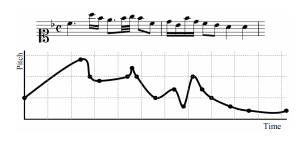
\includegraphics[width=200px,height=100px,keepaspectratio]{one_of_five_point_one}
				\caption{Notes represented as a curve on a pitch-time plane \cite{five_point_two}}
        	\end{figure}
        Based on this principle, Urbano developed two algorithms for the MIREX Competition, Shape (in three variants: ShapeL, ShapeG and ShapeH) which only uses the pitch dimension and Time, which uses both the pitch and the time dimension \cite{five_point_two}. Both algorithms separate melodies into sequences of notes, and use Uniform B-Splines to obtain a spline sequence representation. Two spline sequences are then compared using sequence alignment. Based upon the results of the first Mirex competitions Urbano entered he also developed the ShapeTime system, which collects the n most relevant documents out of the data set, against which the query is run, using the ShapeH system and then ranks those documents using the time system. This was done because the ShapeH system performed better in rank unaware measures, whilst the time system performed better in rank aware measures in the competition. The ShapeTime system usually achieved the best overall results, as we will show later in section 4.2.
        \subsubsection{ShapeH}
        This system ignores the time dimension and only focuses on the shape of a melody. It uses spline-span sequences 3 notes long which results in a polynomial of degree 2 for each spline. These are differentiated next, resulting in polynomials of degree 1. 
        A dynamic programming table is then filled using a global alignment algorithm. The score of a cell (i,j) is computed by : \\
        \begin{center}
            $H(i,j) = max $
            $\begin{Bmatrix*}[c]
            H(i-1, j-1) + s(a_i, b_j) \\
            H(i-1,j) + s(a_i, -) \\
            H(i, j-1) + s(-,b_j)
            \end{Bmatrix*}$
        \end{center}
		where H is the dynamic programming table and a and b the compared spline-span sequences. The highest score from the table is used as the similarity score between the melodies. This prefix-based alignment approach is used in favor of just the global alignment algorithm because Urbano argues that listeners put more emphasis on the beginning of a melody rather than the end when determining similarity. \\
		The operations are defined as follows : 
		
		\begin{center}
            \begin{itemize}
             \item Insertion : 
            $ s(-,n) = -(1-f(n)).$
            \item Deletion : 
             $s(n,-) = -(1 - f(n))$
            \item Match : 
            $s(n,n) = 1-f(n)$
            \end{itemize}
        \end{center}
            
        Where f(n) denotes the relative frequency of a spline in the spline-span sequence. Urbano argues that the more often a spline occurs in the spline-sequence, the less important it is for the comparison. \\
        The substitution or mismatch score is calculated based on the shape of the spans where two melodies with a similar shape only get a small penalization. There are three possible scenarios : 
        \begin{itemize}
         \item If the derivative sign at the start and at the end of the splines are the same, they are considered to have a similar shape and there is only a small penalization.
         \item If the derivative sign only matches at the start or the end of the splines, they are considered to be less similar and there is a medium penalization.
         \item If the derivative sign at the start and the end of the spline does not match, they are considered to be not similar and there is a large penalization.
        \end{itemize}
        Due to looking at polynomials of degree 2 it is sufficient to only regard the start and end points of the splines, because they can only change their direction once within the span.
        It should be noted here that Urbano also submitted the ShapeG and ShapeL systems to Mirex competition until 2013, which only differ from the ShapeH system in that they use a strictly global and a strictly local alignment approach, respectively, instead of the hybrid alignment approach. However the ShapeH system on average produced the best results in the Mirex competitions as we will show in section 4.2.
  
		
		\subsubsection{Time}
        \begin{figure}[h!]
			\centering
		  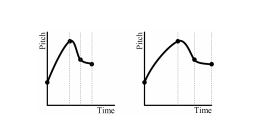
\includegraphics[width=200px,height=100px,keepaspectratio]{two_of_five_point_one}
			\caption{Normalization of spline \cite{five_point_two}}
        \end{figure}
        This system also uses the time dimension and calculates the area between splines to determine similarity. It uses spline-span sequences 4 notes long which results in a polynomial of degree 3 for each spline. They are differentiated, resulting in polynomials of degree 2. Each span duration is normalized to the same length (Fig 2). It uses the same hybrid alignment approach as the ShapeH system. 
		The operations are defined as follows : 
        \begin{itemize}
         \item Insertion : 
        $ s(-,n) = -diff _p(n, \phi(n)) - \lambda k_t * diff_t(n, \phi(n)).$
        \item Deletion : 
         $s(n,-) = -diff_p(n, \phi(n)) - \lambda k_t * diff_t (n, \phi(n)).$
       \item substitution : 
       $s(n,m) = - diff_p (n,m) - \lambda k_t * diff_t (n,m) $
       \item Match : 
        $s(n,n) = 2\mu_p + 2\lambda k_t \mu_t = 2\mu_p (1+k_t).$
        \end{itemize}
        
        $diff_p$ and $diff_t$ are defined as the area between the first derivatives from the splines pitch and time function. $ \phi(n)$ describes the area between n and the x-axis. $\mu_p$, $\mu_t$ as well as $k_t$ are weighting constants where $\mu_p$ and $\mu_t$ being the mean scores returned by $diff_p$ and $diff_t$ respectively and $k_t$ weighing time dissimilarity corresponding to pitch dissimilarity. $ \lambda = \mu_p / \mu_t$ is a constant used to normalize time distance with respect to pitch distance.
        
	\section{MIREX}
		MIREX is a platform for researchers in Music IR. It organizes annual competition where researchers present their algorithms. The subbranch "Symbolic Melodic Music Similarity" was active during 2005-2015 and doesn't anymore take place since then. 

		As we mentioned in the introduction, one of the main problems of Symbolic Melodic Music Similarity is that there is no consensus over a universal measure of similarity. In order to circumvent this issue, MIREX consults ratings given by experts of the field. The results of the competitors were compared against this so-called Ground Truth.
		
		\subsection{The Ground Truth}
 		The RISM A/II collection, which was used as the collection in the competition of 2005, contains 476,000 documents. Experts were asked to rate similarity of documents in this collection to given queries. The experts were not asked to evaluate similarity to all documents, since that would take too much time. A series of filtering processes were applied to reduce the number of relevant documents. 

 		Among several of them melodies were filtered based on: 

 		\begin{itemize}
 			\item The interval between the highest and lowest note within the melody
 			\item The largest interval between subsequent notes.
 			\item The editing distance between the query and the document. In order to find the editing distance, a document is projected onto a string, that contains the alphabet U("up"), D("down"), R("repeat"). 
 		\end{itemize} 

        Interval in music means, the distance between two notes, that specifies its relation between 2 notes in terms of the number of half-steps between them if they are ordered in an ascending order or descending.
	    
 		Different filtering steps are used based on characteristic features of the documents. In order to prevent relevant documents from being filtered out, a limit of 300 documents was set. To come to a convenient number of documents, 300 documents were then manually reduced to a collection of 50 documents.

 		The relevant documents were then given to the experts to be ordered with respect to a query. Experts were given the freedom to choose which documents were to be included at all. The rankings were grouped together for each document, ordered by their by median rank and then by mean rank. Every document is then compared against higher ranked documents by Wilcoxon rank sum test, that measures the probability of the null-hypothesis, that is, the probability that the ratings of a relatively small group of experts reflect those of a larger group. When there is no compelling evidence that documents actually differ in terms of median ranks, they are ranked equally. As a consequence of this there is often no total order among ranked documents. 

 		\begin{figure}[h!]
			\centering
			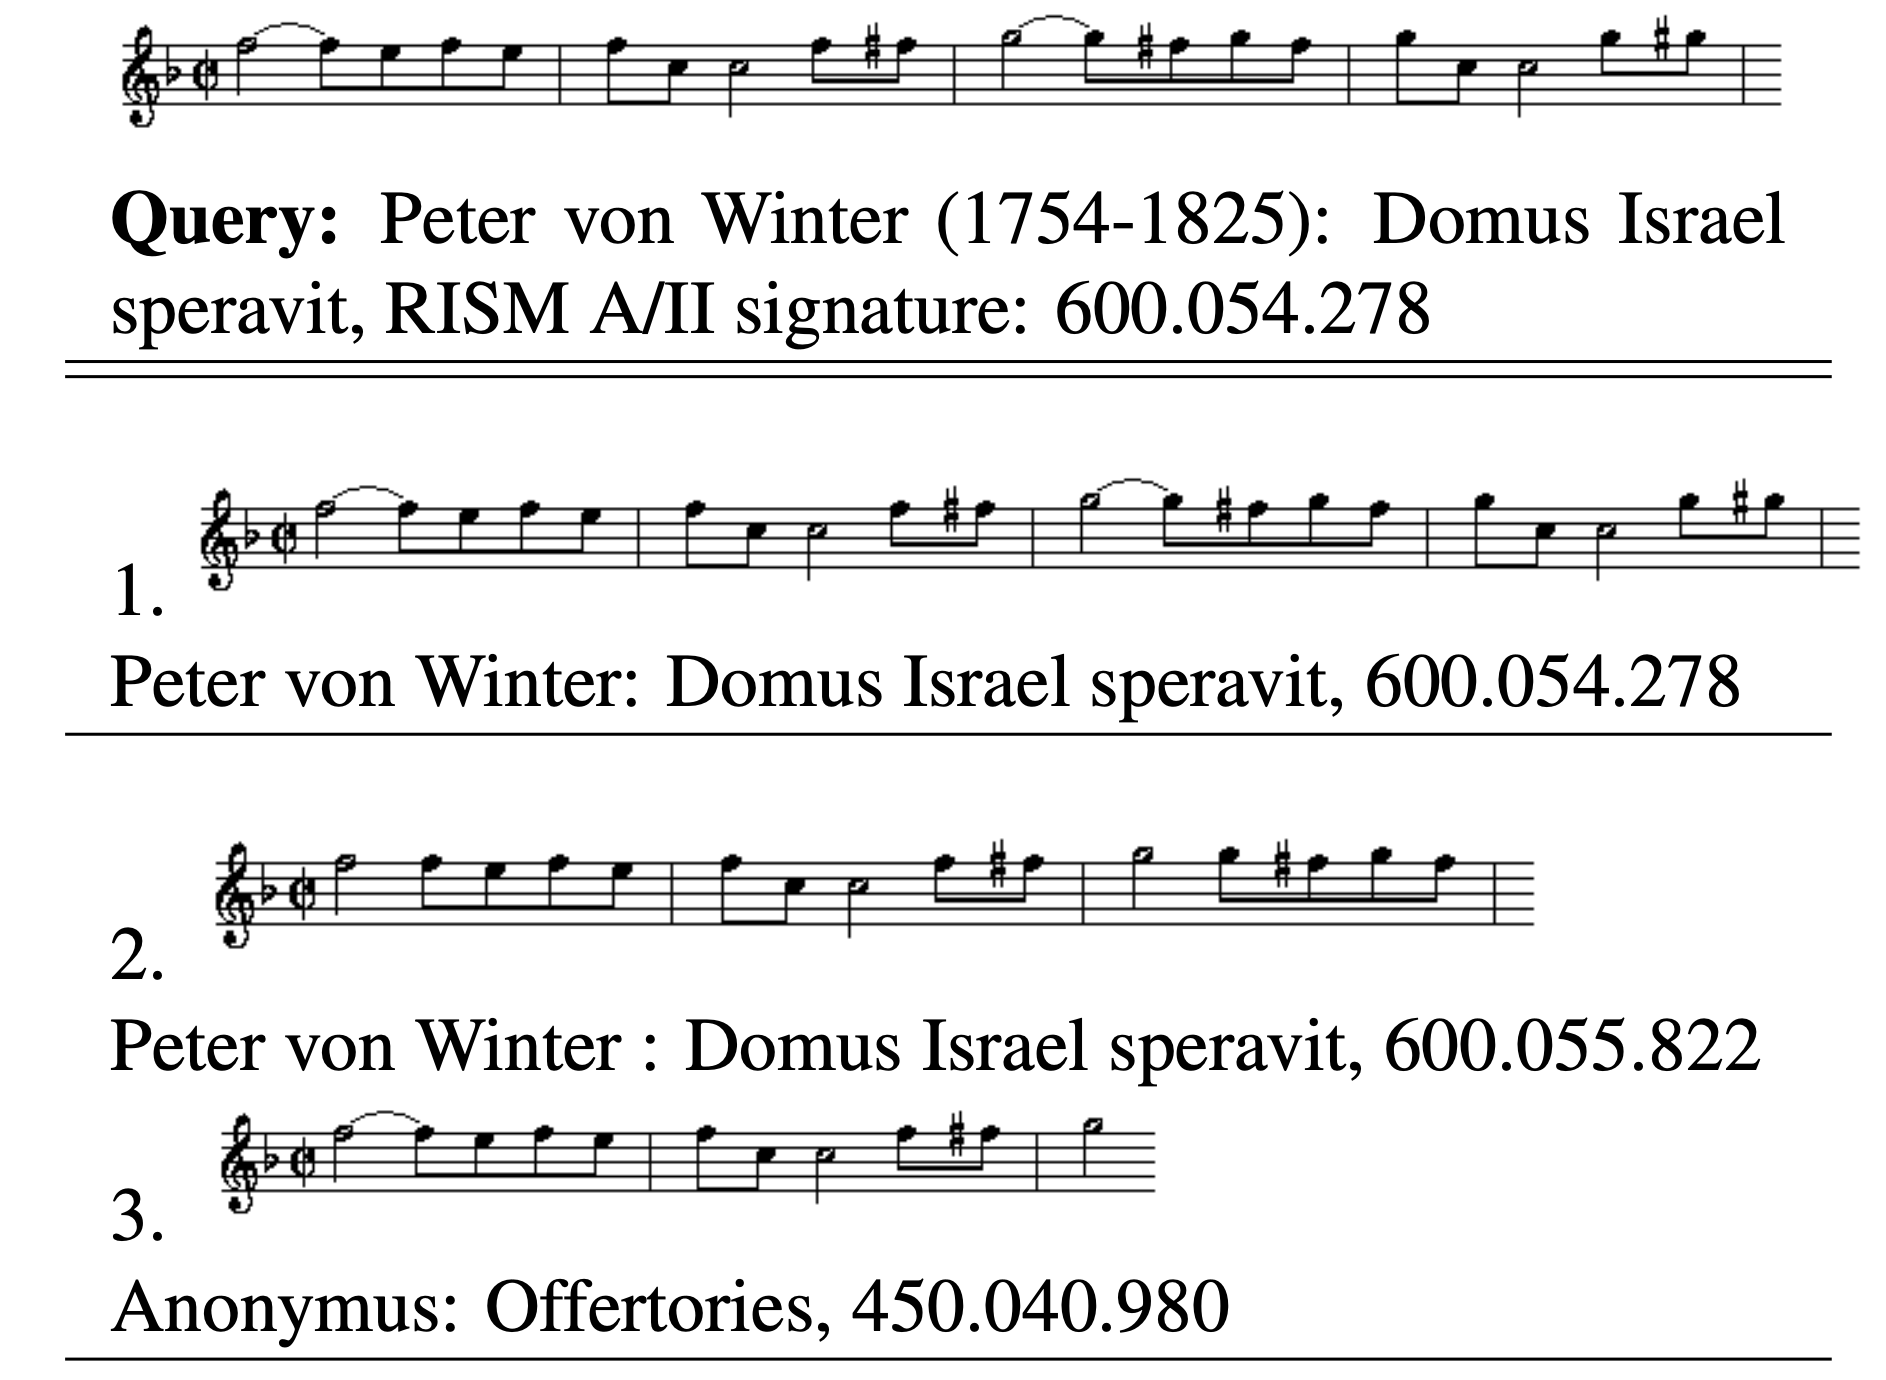
\includegraphics[width=200px,height=100px,keepaspectratio]{one_of_two_point_four_point_four}
			\caption{Ground Truth for Winter: “Domus Israel speravit" \cite{two_point_four_point_four}}
		\end{figure}


 		 In \cite{two_point_four_point_four} 31 experts were asked to order relevant documents to the given query in \textbf{Fig. 3}. The second and the third documents in the resulting list differ from the given query in such small ways, that it was hard to conclude a total order among results.

		\subsection{Average Dynamic Recall}

			To emphasize the group boundaries better, Typke, Veltkamp, Wiering \cite{three}introduces a new measure called Average Dynamic Recall. The authors mention nine criteria that they considered when they introduced ADR, among which we are :

			\begin{itemize}
				\item The measure doesn't need the ground truth to be completely ordered
				\item Violations of the correct order should be punished if they happen across group boundaries.
			\end{itemize}

			In comparison to standard measures such as recall and precision, ADR is specifically tailored for partially ordered lists.
			The ADR is calculated as the sum of recall over number of iterations. The relevant documents  at the beginning are the  documents within the first group. When this group of elements is completely retrieved, the number of relevant documents will get larger by adding the next group about which it is known that there is evidence that documents do differ in terms of median ranks. In each step the recall is calculated as the ratio of found currently relevant documents over the number of currently relevant documents.

			
	\section{Evaluation}
		\subsection{The graph based algorithm of Orio et al.}
			For the evaluation shown in Fig. 4 authors used the RISM A/II collection with Ground Truth and queries from MIREX 2005 \cite{three}.
			
			\begin{figure}[h!]
			\centering
			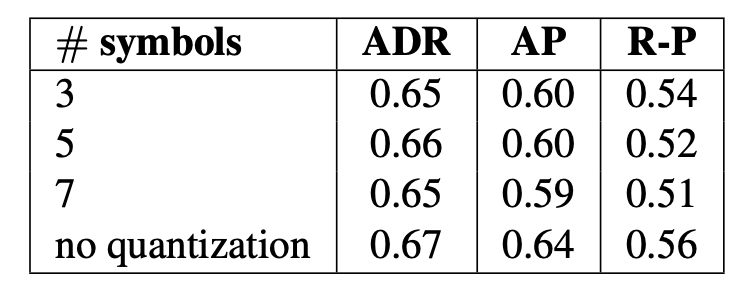
\includegraphics[width=200px,height=100px,keepaspectratio]{one_of_two_point_four}
			\caption{Manual segmentation using projections with ranges of different sizes.\cite{two_point_four} ADR is explained in Chapter 3 , AP is averaged precision and R-P is R-Precision.}
			\end{figure}
            
            Authors experimented with the input data to see what impact it would have if the melodies were to be projected to simpler melodies, which still reflect basic elements of the starting melody. Figure 4 shows the averaged results of the algorithm when using quantization with alphabets of various sizes. Quantization can be seen as a function that projects a given melody onto a sequence of symbols. An example to a quantization with 3 symbols is a function that projects a melody onto the alphabet ('up','down','repeat'). We observe that reducing a melody into a simpler melody, results in loss of result quality, though often not significant enough for success of retrieval. Authors mention that \textit{"this aspect should be investigated in more detail with a larger collection because a coarse quantization allows us to reduce the size of the PSR improving efficiency"}.

			\begin{figure}[h!]
			\centering
			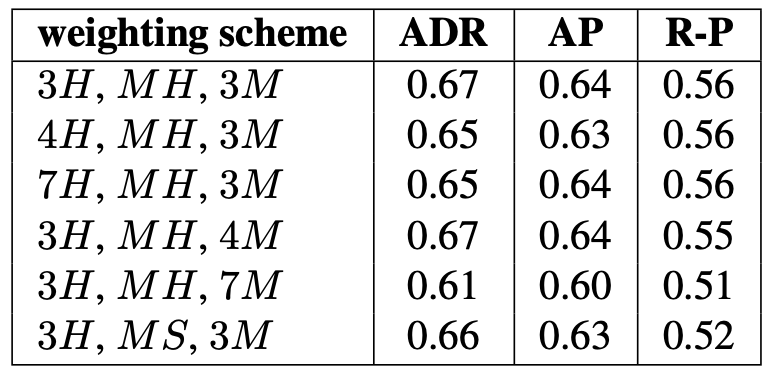
\includegraphics[width=200px,height=100px,keepaspectratio]{three_of_two_point_four}
			\caption{Different segmentation techniques with no quantization \cite{two_point_four}}
			\end{figure}

			Figure 2 shows use of different weight measures. As mentioned in section 2.1 weight measures are important for choosing the more important note among other notes in a measure. For harmonic weight the authors experimented with different alphabets size 3,4 and 7. An example to an alphabet of size 3 would consist in grouping the first, fourth and sixth degrees to a group, grouping second and seventh to another and rest to the third group. How these groupings are formed is based on Music Theory. The projection of a single note in the starting melody is based upon its harmonic meaning within the musical context. While reducing the different harmonic functionalities into one larger group, it is important to make assumptions, that lead to a grouping with the least amount of information loss. With the same consideration melodic weights have  been grouped together as well. As to metric weight, there are two different schemes that have been proposed by authors : (1) A simple subdivision in terms of strong and weak beats and (2) \textit{"a hierarchical organization depending on the position in the measure"}. In Fig 5 we observe that, even though the differences are not significant enough, the better results are obtained when weighting is based on more generalizing schemes.
			
			\begin{figure}[h!]
			\centering
            \includegraphics[width=350px,height=160px,keepaspectratio]{four_of_five_point_five}
			\caption{Number of new added documents to the tree when new documents are added to it. \cite{five_point_five}}
        	\end{figure}

			The generalization processes that graph based algorithm use are highly dependent upon annotations of harmonic functions of melodic data, which are rarely included in symbolic melodic data. Authors see this as a drawback since a false assumption of a harmonic function of a note in input could easily result in a false segmentation of a piece within. As it can be seen in Fig. 5 the tree that is formed as musical data are added to it has a tendency to grow in sublinear fashion. We see this sublinear tendency as an advantage for memory consumption.

  \subsection{Urbano Melody-Shape}
            In the initial paper of 2010 \cite{five_point_five}, where Urbano et al. first proposed to compare melodies based on their shape, the authors tested their implementation using the RISM A/II collection from MIREX 2005 and compared their results to the results of the competing algorithms from 2005 . As can be seen in Fig 6(Splines column), their Spline-based implementation performed best in 5 out of 11 queries  and averaged the highest ADR score overall. 
        \begin{figure}[h!]
			\centering
            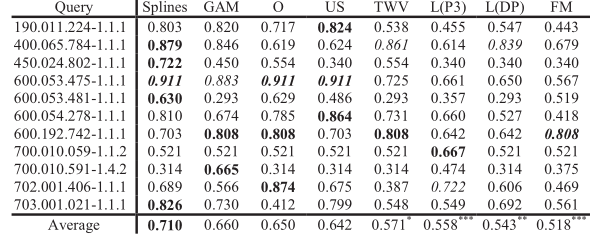
\includegraphics[width=350px,height=160px,keepaspectratio]{one_of_five_point_five}
			\caption{Spline based approach tested against the evaluation set of the MIREX 2005 competition and compared to the other contestants. \cite{five_point_five}}
        \end{figure}
            The algorithm used was later improved upon and very similar to the time system we presented earlier, using the area between two splines and a local alignment approach to determine similarity. Based upon this system Urbano developed the ShapeH and Time systems  and competed in the 2010-2015 editions of the MIREX Competition, with all submitted systems always placing in the top spots. \cite{five_point_six}\cite{five_point_seven}\cite{five_point_four}
            \cite{five_point_three}
            \cite{five_point_two}
            \cite{five_point_eight}
        \begin{figure}[h!]
			\centering
            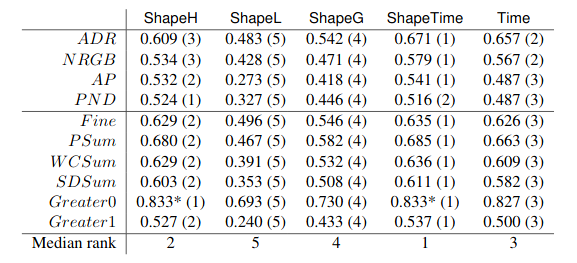
\includegraphics[width=250px,height=125px,keepaspectratio]{urbano_mirex_2012_results}
			\caption{Results for the submissions by Urbano to the 2012 MIREX Competition \cite{five_point_four}}
        \end{figure}
        \begin{figure}[h!]
			\centering
            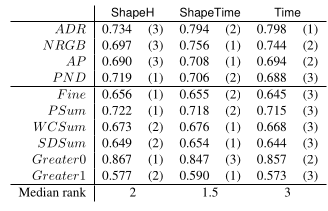
\includegraphics[width=200px,height=100px,keepaspectratio]{urbano_mirex_2013_results}
			\caption{Results for the submissions by Urbano to the 2013 MIREX Competition \cite{five_point_three}}
        \end{figure}
        \begin{figure}[h!]
			\centering
            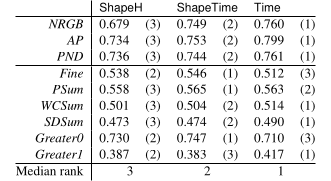
\includegraphics[width=200px,height=100px,keepaspectratio]{urbano_mirex_2014_results}
			\caption{Results for the submissions by Urbano to the 2014 MIREX Competition \cite{five_point_two}}
        \end{figure}
        
        However although the systems by Urbano seem to perform best in the competition, the results themselves vary from year to year with the algorithms not really having changed, as Urbano himself points out in his paper to the 2014 competition \cite{five_point_two}.  While the ShapeTime system, as mentioned in section 2.2, usually achieved the best results on average, it was outperformed by the time system in 2014 (Fig.9). Scores in single categories also varied with the ShapeH system achieving an ADR score of 0.609 in the 2012 competition (Fig.7) and achieving a a score of 0.734 in the same category the following year (Fig.8). 


	\section{Discussion}
	
	There still seem to be  several problems in the field of symbolic melodic music similarity.
	There is no definitive definition for what exactly constitutes music similarity and no agreed upon data set exists, against which methods can be evaluated. This makes comparing different methods challenging, if not impossible. Even the results from different years of the MIREX competitions cannot really be compared to each other, as the scoring appears to be inconsistent. Furthermore the used queries and corresponding Ground Truth have not been released since 2010, effectively making comparing a new method to the results from the competition impossible. There are also only limited real world applications for algorithms that only compare monophonic pieces, as most music consists of polyphonic compositions. We think that due to these reasons advancement in the field of Symbolic Melodic Music Similarity has slowed down in recent years, with the MIREX competition not listing the subcategory since 2016 as well.


	\begin{comment}
		TODO: This was before in Introduction . But Herr Leser wanted us to put this into conclusion. Okay , but how?
		
		Our main emphasis is that the field suffers from the subjectivity of music similarity with no agreed upon definition existing of what constitutes similarity between pieces of music. Many algorithms lack empirical evaluation and with no Ground Truths existing, the data that does exist is very hard to compare.
	\end{comment}


	\begin{thebibliography}{7}
	
	\bibitem {kil:civ}
	A. D. Kilmer and M. Civil, 
	"Old Babylonian Musical Instructions Relating to Hymnody" 
	Journal of Cuneiform Studies 38, 
	no. 1 (Spring 1986): 94-98.

	\bibitem{five_point_two} 
	J. Urbano. MelodyShape at 
	MIREX 2014 Symbolic Melodic Similarity. 
	Technical report, Music Information Retrieval Evaluation eXchange, 2014.

	\bibitem{two}
	Symbolic Melodic Similarity: State of the Art and Future Challenges
	Valerio Velardo,Mauro Vallati and Steven Jan
	Computer Music Journal, 40:2, pp. 70–83, Summer 2016 doi:10.1162/COMJ a 00359
	2016, Massachusetts Institute of Technology.v

	\bibitem{two_point_four} Orio, N., and A. Rodá. 2009. “A Measure of Melodic Similarity Based on a Graph Representation of the Music Structure.” In Proceedings of the International Conference for Music Information Retrieval, pp. 543– 548.

	\bibitem{three} Typke, Rainer. (2007). Music Retrieval based on Melodic Similarity.

	\bibitem{one} Greg Aloupis, Thomas Fevens, Stefan Langerman, Tomomi Matsui, Antonio Mesa, Yurai Nunez, David Rappaport, and Godfried Toussaint, "Algorithms for Computing Geometric Measures of Melodic Similarity" Computer Music Journal, Vol.30, No. 3 (Autumn, 2006), pp. 67-76

	\bibitem{two_point_four_point_four} R. Typke, R. C. Veltkamp and F. Wiering, "A Measure for Evaluating Retrieval Techniques based on Partially Ordered Ground Truth Lists," 2006 IEEE International Conference on Multimedia and Expo, Toronto, Ont., 2006, pp. 1793-1796.
	
	\bibitem{five_point_five} J.Urbano, J. Morato, J. Lloréns, S. Sanchez Cuadrado, "Using the Shape of Music to Compute the Similarity between Symbolic Musical Pieces", International Symposium on Computer Music Modeling and Retrieval, pp. 385-396, 2010
	
	\bibitem{five_point_three} J. Urbano. MIREX 2013 Symbolic Melodic Similarity:
	A Geometric Model supported with Hybrid Sequence
	Alignment. Technical report, Music Information Retrieval Evaluation eXchange, 2013.

 	\bibitem{five_point_four} J. Urbano, J. Lloréns, J. Morato, and S. Sánchez 
	Cuadrado. MIREX 2012 Symbolic Melodic Similar-
	ity: Hybrid Sequence Alignment with Geometric Rep-
	resentations. Technical report, Music Information Re-
	trieval Evaluation eXchange, 2012.

    \bibitem{five_point_six} J. Urbano, J. Lloréns, J. Morato, and S. Sánchez 
	Cuadrado "MIREX 2010 Symbolic Melodic Similarity: Local alignment with geometric representations", Music Information Retrieval Evaluation eXchange, 2010.
    \bibitem{five_point_seven} J. Urbano, J. Lloréns, J. Morato, and S. Sánchez 
	Cuadrado, "MIREX 2011 Symbolic Melodic Similarity: Sequence alignment with geometric representations", Technical report, Music Information Re-
	trieval Evaluation eXchange, 2011.
    \bibitem{five_point_eight} J. Urbano. MelodyShape at MIREX 2015 Symbolic Melodic Similarity. Technical report, Music Information Retrieval Evaluation eXchange, 2015.
	\bibitem{six} Karaosmanoğlu, M. Kemal , "A TURKISH MAKAM MUSIC SYMBOLIC DATABASE FOR
	MUSIC INFORMATION RETRIEVAL: SymbTr" , 13th International Society for Music Information Retrieval , 2012.
	

	\end{thebibliography}

	
\end{document}
